\section{Matching}
\begin{definition}[Matching]~
	\begin{itemize}
		\item[i)] Ein \textbf{Matching} in einem Grap $G=(V,E)$ ist eine Menge paarweise disjunkter Kanten.
		\item[ii)] Ein Matching heißt \textbf{perfekt}, wenn jeder Knoten in $V(G)$ zu einer Matchingkante gehört.
		\item[iii)] Ein \textbf{Vertex Cover} ist eine Kantenüberdeckende Knotenmenge.
		\item[iv)] \textbf{Maximales Matching} in $G:$ $\mathcal{V}(G)$.
		\item[v)] \textbf{Minimales Vertex Cover} in $G:$ $\mathcal{T}(G)$.
	\end{itemize}
\end{definition}
\begin{figure}[ht]
	\begin{subfigure}[c]{0.5\textwidth}
		\begin{center}
			\begin{tikzpicture}
			\node[circle, fill, blue, scale = .8] (A) {};
			\node[circle, fill, black, scale = .8, below = 0.5cm of A] (B) {};
			\node[circle, fill, blue, scale = .8, below = 0.5cm of B] (C) {};
			\node[circle, fill, black, scale = .8, below = 0.5cm of C] (D) {};
			\node[circle, fill, blue, scale = .8, below = 0.5cm of D] (E) {};
			\node[circle, fill, blue, scale = .8, below = 0.5cm of E] (F) {};
			
			\node[circle, fill, black, scale = .8, right = 3cm of A] (H) {};
			\node[circle, fill, black, scale = .8, below = 0.5cm of H] (I) {};
			\node[circle, fill, blue, scale = .8, below = 0.5cm of I] (J) {};
			\node[circle, fill, black, scale = .8, below = 0.5cm of J] (K) {};
			\node[circle, fill, blue, scale = .8, below = 0.5cm of K] (L) {};
			\node[circle, fill, black, scale = .8, below = 0.5cm of L] (M) {};
			
			\path (A) edge (H);
			\path (A) edge (I);
			\path (B) edge (J);
			\path (C) edge (H);
			\path (C) edge (J);
			\path (C) edge (K);
			\path (D) edge (L);
			\path (E) edge (H);
			\path (E) edge (I);
			\path (E) edge (J);
			\path (E) edge (K);
			\path (E) edge (L);
			\path (E) edge (M);
			\path (F) edge (L);
			\path (F) edge (M);
			\end{tikzpicture}
		\end{center}
		\subcaption{Vertex Cover}
	\end{subfigure}
	\begin{subfigure}[c]{0.5\textwidth}
		\begin{center}
			\begin{tikzpicture}[every loop/.style={}]
			\node[circle, fill, black, scale = .8] (A) {};
			\node[circle, fill, black, scale = .8, below = 0.5cm of A] (B) {};
			\node[circle, fill, black, scale = .8, below = 0.5cm of B] (C) {};
			\node[circle, fill, black, scale = .8, below = 0.5cm of C] (D) {};
			\node[circle, fill, black, scale = .8, below = 0.5cm of D] (E) {};
			\node[circle, fill, black, scale = .8, below = 0.5cm of E] (F) {};
			
			\node[circle, fill, black, scale = .8, right = 3cm of A] (H) {};
			\node[circle, fill, black, scale = .8, below = 0.5cm of H] (I) {};
			\node[circle, fill, black, scale = .8, below = 0.5cm of I] (J) {};
			\node[circle, fill, black, scale = .8, below = 0.5cm of J] (K) {};
			\node[circle, fill, black, scale = .8, below = 0.5cm of K] (L) {};
			\node[circle, fill, black, scale = .8, below = 0.5cm of L] (M) {};
			
			\path (A) edge (I);
			\path (B) edge (J);
			\path (C) edge (H);
			\path (D) edge (L);
			\path (E) edge (K);
			\path (F) edge (M);
			\end{tikzpicture}
		\end{center}
		\subcaption{Matching}
	\end{subfigure}
	\caption{Vertex Cover und Matching im bipartiten Graph}
\end{figure}
\begin{problem}[Kardinalitätsmatching/Max Matching]~\\[5pt]
	\hspace*{10pt}\textbf{Gegeben: }Ungerichteter Graph $G = (V,E)$.\\[5pt]
	\hspace*{10pt}\textbf{Gesucht: }Ein Matching $M$ größtmöglicher Kardinalität.
\end{problem}
\begin{problem}[Minimales Vertex Cover]~\\[5pt]
	\hspace*{10pt}\textbf{Gegeben: }Ungerichteter Graph $G = (V,E)$.\\[5pt]
	\hspace*{10pt}\textbf{Gesucht: }Ein Vertex Cover $C$ kleinstmöglicher Kardinalität.
\end{problem}
\begin{satz}
	Sei $G$ ein ungerichteter Graph. Es gilt max Matching $\le$ min Vertex Cover.
\end{satz}
\begin{figure}[ht]
	\begin{center}
		\begin{tikzpicture}
			\node[circle, fill, black, scale = .8] (A) {};
			\node[circle, fill, blue, scale = .8, below left = 1cm of A] (B) {};
			\node[circle, fill, blue, scale = .8, below right = 1cm of A] (C) {};
			
			\path (A) edge[red] (B);
			\path (A) edge (C);
			\path (B) edge (C);
		\end{tikzpicture}
		\end{center}
	\caption{max Matching $\le$ min Vertex Cover}
\end{figure}
\newpage
\subsection{Bipartites Matching}
\begin{definition}[Bipartite Graphen]
	Ein Graph heißt \textbf{bipartit}, wenn sich die Knotenmenge so in zwei Mengen $A,B$ mit $V(G) = A \dot\cup B$ zerlegen lässt, dass jede Kante genau einen Knoten in $A$ und einen Knoten in $B$ enthält.
\end{definition}
\textit{Damit: Bipartite Graphen enthalten keine Kreise ungerader Länge. Für bipartite Graphen gibt es eine Beziehung zu Flussproblemen:}
\begin{center}
	\begin{tikzpicture}
		\node[circle, fill, black, scale = .8] (A) {};
		\node[circle, fill, black, scale = .8, below = .5cm of A] (B) {};
		\node[circle, fill, black, scale = .8, below = .5cm of B] (C) {};
		\node[circle, fill, black, scale = .8, below = .5cm of C] (D) {};
		
		\node[circle, fill, black, scale = .8, right = 2cm of A] (E) {};
		\node[circle, fill, black, scale = .8, below = .5cm of E] (F) {};
		\node[circle, fill, black, scale = .8, below = .5cm of F] (G) {};
		\node[circle, fill, black, scale = .8, below = .5cm of G] (H) {};
		\node[circle, fill, black, scale = .8, below = .5cm of H] (I) {};
		
		\path (A) edge (E);
		\path (B) edge (E);
		\path (B) edge (F);
		\path (C) edge (G);
		\path (C) edge (H);
		\path (C) edge (I);
		\path (D) edge (F);
	\end{tikzpicture}
\end{center}
\textit{
\begin{itemize}
	\item füge 2 neue Knoten $s,t$ ein: Kanten von $s$ nach $v\in A$ und von $v\in B$ zu $t$.
	\item Kanten von $A$ nach $B$ richten.
	\item $u(e) = 1$ falls $s\in e$ oder $t\in e$, $u(e) = \infty$ sonst.
\end{itemize}
}
\begin{center}
	\begin{tikzpicture}
	\node[circle, fill, black, scale = .8, below left = 1.5cm of A, label = s] (S) {};
	\node[circle, fill, black, scale = .8] (A) {};
	\node[circle, fill, black, scale = .8, below = .5cm of A] (B) {};
	\node[circle, fill, black, scale = .8, below = .5cm of B] (C) {};
	\node[circle, fill, black, scale = .8, below = .5cm of C] (D) {};
	
	\node[circle, fill, black, scale = .8, below right = 1.5cm of E, label = t] (T) {};
	\node[circle, fill, black, scale = .8, right = 2cm of A] (E) {};
	\node[circle, fill, black, scale = .8, below = .5cm of E] (F) {};
	\node[circle, fill, black, scale = .8, below = .5cm of F] (G) {};
	\node[circle, fill, black, scale = .8, below = .5cm of G] (H) {};
	\node[circle, fill, black, scale = .8, below = .5cm of H] (I) {};
	
	\path (A) edge[->] node[above, scale = .8]{$\infty$} (E);
	\path (B) edge[->] node[above, scale = .8]{$\infty$} (E);
	\path (B) edge[->] node[above, scale = .8]{$\infty$} (F);
	\path (C) edge[->] node[above, scale = .8]{$\infty$} (G);
	\path (C) edge[->] node[above, scale = .8]{$\infty$} (H);
	\path (C) edge[->] node[above, scale = .8]{$\infty$} (I);
	\path (D) edge[->] node[above, scale = .8]{$\infty$} (F);
	\path (S) edge[->] node[above, scale = .8]{1} (A);
	\path (S) edge[->] node[above, scale = .8]{1} (B);
	\path (S) edge[->] node[above, scale = .8]{1} (C);
	\path (S) edge[->] node[above, scale = .8]{1} (D);
	\path (E) edge[->] node[above, scale = .8]{1} (T);
	\path (F) edge[->] node[above, scale = .8]{1} (T);
	\path (G) edge[->] node[above, scale = .8]{1} (T);
	\path (H) edge[->] node[above, scale = .8]{1} (T);
	\path (I) edge[->] node[above, scale = .8]{1} (T);
	\end{tikzpicture}
\end{center}
\textit{Aus gegebenen bipartiten Graph $G$ wird $(G',u,s,t)$.}
\begin{satz}
	Ein bipartites Matching maximaler Kardinalität in $G$ entspricht einem maximalen Fluss in $(G',u,s,t)$ und umgekehrt.
\end{satz}
\begin{proof}~
	\begin{itemize}
		\item Jedes Matching in $G$ lässt sich direkt auf einen Fluss in $G'$ abbilden, indem die Matchingkanten einen Fluss von jeweisl 1 erhalten und entsprechende Flüsse von $s$ und $t$ gewählt werden.
		\item Umgekehrt lässt sich jeder ganzzahliger Fluss (der auf jeder Kante den Wert 0 oder 1 hat) auf ein Matching in $G$ abbilden.
	\end{itemize}
	Da es immer ein ganzzahliges Optimum für das Flussproblem gibt, sind also insbesondere die Optimalwerte gleich.
\end{proof}
\begin{satz}
	In bipartiten Graphen gilt $\mathcal{V}(G) = \mathcal{T}(G)$.
\end{satz}
\begin{proof}
	$\mathcal{V}(G) = Max~Flow(G) = Min~Cut(G) \overset{!}{=} \mathcal{T}(G)$. 
		\begin{figure}[ht]
			\begin{center}
				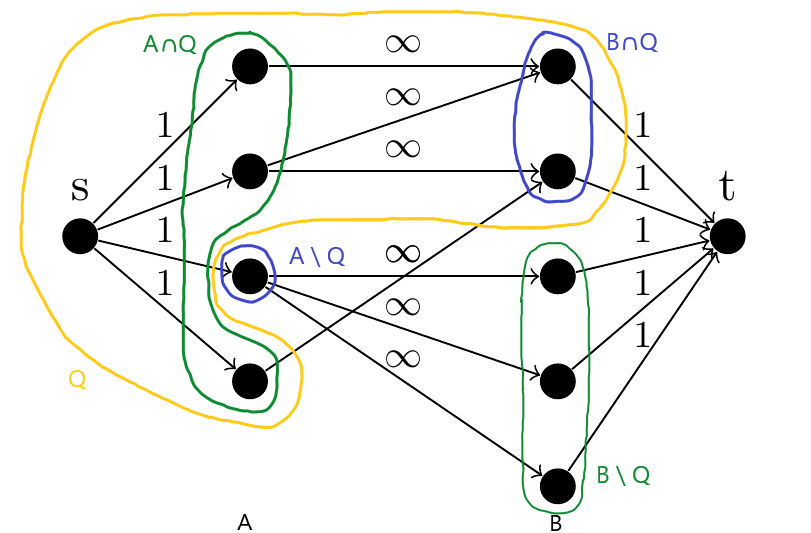
\includegraphics[scale=.3]{satz_5_8.png}
			\end{center}
		\end{figure}\\
	Betrachte Min Cut $\delta^+(\set{s}\cup Q), Q \subseteq V$. Dieser Cut hat endliche Kapazität, d.h. es gibt keine Kante von $A \cap Q$ zu $B\setminus Q$.
	\begin{eqnarray*}
		A \cap Q & \text{ zu } & B \cap Q\\
		A \cap Q & \text{ zu } & B \setminus Q ~\lightning\\
		A \setminus Q & \text{ zu } & B \cap Q\\
		A \setminus Q & \text{ zu } & B \setminus Q
	\end{eqnarray*}
	Also ist jede Kante in $G$ inzident zu einem Knoten aus $C = (A\setminus Q)\cup (B \cap Q)$. D.h. $C$ ist ein Cover der Größe $\card{C} = \card{A\setminus Q} + \card{B\cap Q}$. Die Kapazität des Cuts ist ebenfalls $\card{C} = \card{A\setminus Q} + \card{B\cap Q}$ (nach Konstruktion) d.h. Min Cut = min Vertex Cover.
\end{proof}
\begin{satz}[Satz von Hall]
	Sei $G$ ein bipartiter Graph mit $V(G)=A\dot\cup B$. Dann hat $G$ ein $A$ überdeckendes Matching $\Leftrightarrow$ $\card{\underbrace{T(X)}_{\mathclap{\text{Menge der Nachbarn von } X}}} \ge \card{X}~\forall X\subseteq A$.
\end{satz}
\begin{proof}~
	\begin{itemize}
		\item Notwendigkeit ist klar.
		\item Um zu zeigen, dass auch hinreichend nehmen wir an $G$ hat kein $A$ überdeckendes Matching. $\mathcal{V}(G) \le \card{A} \overset{5.7}{\Rightarrow} \mathcal{T}(G) < \card{A}$. Sei $A' \subseteq A, B' \subseteq B$, so dass $A' \cup B'$ alle Kanten überdeckt und $\card{A' \cup B'} < \card{A} \Leftrightarrow \card{A'} + \card{B'} < \card{A}$ (da $A'$ und $B'$ disjunkt) $\Leftrightarrow \card{B'} < \card{A} - \card{A'}$. Es gilt $T(A\setminus A') \subseteq B'$ ( da $B'$ alle Kanten überdeckt, die nicht von $A'$ überdeckt werden) $\Rightarrow \card{T(A\setminus A')} \le \card{B'} < \card{A} - \card{A'} = \card{A\setminus A'}~\lightning$ Kontraposition der Hinrichtung gezeigt.
	\end{itemize}
\end{proof}
\begin{korollar}[Heiratssatz von Frobenius]
	Sei $G$ ein bipartiter Graph mit $V(G) = A\dot\cup B$. Dann hat $G$ ein perfektes Matching $\Leftrightarrow \card{A}=\card{B}$ und $\card{T(X)} \ge \card{X}~\forall X \subseteq A$.
\end{korollar}
\textit{Aus dem Beweis von Satz 5.7 folgt}
\begin{korollar}
	Das Kardinalitätsmatching-Problem kann in bipartiten Graphen in $O(n\cdot m)$ gelöst werden.
\end{korollar}
\begin{proof}
	Konstruktion von oben. Betrachte Ford-Fulkerson für das äquivalente Flussproblem
	\begin{itemize}
		\item Eine Augmentierung benötigt $O(m)$.
		\item Um einen maximalen $s$-$t$-Fluss (und damit ein maximales Matching) zu finden brauchen wir höchstens $n$ Augmentierungen $\Rightarrow$ $(O(m\cdot n))$.
	\end{itemize}
\end{proof}
\textit{Wie sehen Augmentierungen aus?\\
\hspace*{10pt}$\hookrightarrow$ Verbesserung von Matchings}
\begin{figure}[ht]
	\begin{center}
	\begin{tikzpicture}
	\node[circle, fill, black, scale = .8, below left = 1.5cm of A, label = s] (S) {};
	\node[circle, fill, black, scale = .8] (A) {};
	\node[circle, fill, black, scale = .8, below = .5cm of A] (B) {};
	\node[circle, fill, black, scale = .8, below = .5cm of B] (C) {};
	\node[circle, fill, black, scale = .8, below = .5cm of C] (D) {};
	
	\node[circle, fill, black, scale = .8, below right = 1.5cm of E, label = t] (T) {};
	\node[circle, fill, black, scale = .8, right = 2cm of A] (E) {};
	\node[circle, fill, black, scale = .8, below = .5cm of E] (F) {};
	\node[circle, fill, black, scale = .8, below = .5cm of F] (G) {};
	\node[circle, fill, black, scale = .8, below = .5cm of G] (H) {};
	
	\path (A) edge[->] (E);
	\path (B) edge[->, red] (E);
	\path (B) edge[->] (F);
	\path (C) edge[->] (G);
	\path (C) edge[->, red] (F);
	\path (D) edge[->, red] (G);
	\path (D) edge[->] (H);
	\path (S) edge[->] (A);
	\path (S) edge[->] (B);
	\path (S) edge[->] (C);
	\path (S) edge[->] (D);
	\path (E) edge[->] (T);
	\path (F) edge[->] (T);
	\path (G) edge[->] (T);
	\path (H) edge[->] (T);
	
	\path (S) edge[->, green, bend left] (A);
	\path (A) edge[->, green, bend left] (E);
	\path (E) edge[->, green, bend right] (B);
	\path (B) edge[->, green, bend left] (F);
	\path (F) edge[->, green, bend right] (C);
	\path (C) edge[->, green, bend left] (G);
	\path (G) edge[->, green, bend right] (D);
	\path (D) edge[->, green, bend right] (H);
	\path (H) edge[->, green, bend right] (T);
	\end{tikzpicture}
	\caption{augmentierender Pfad in $G'$}
	\end{center}
\vspace*{-10pt}
\end{figure}\\
\textit{Augmentierende Pfade in $(G',u,s,t)$ entsprechen alternierenden Pfaden in $G$.}
\begin{definition}
	Sei $G$ ein Graph (bipartit oder nicht), und sei $M$ ein beliebiges Matching in $G$. Ein Pfad $P$ ist ein \textbf{$M$-alternierender Pfad}, wenn $E(P)\setminus M$ ein Matching ist. Ein $M$-alternierender Pfad ist \textbf{$M$-augmentierend}, wenn seine Endpunkte nicht von $M$ überdeckt werden (er zwei nicht gematchte Knoten verbindet).
\end{definition}
\textit{Augmentierende Pfade müssen ungerade Länge haben.}
\begin{figure}[ht]
	\begin{center}
	\begin{tikzpicture}
	\node[circle, fill, black, scale = .8] (A) {};
	\node[circle, fill, black, scale = .8, right = .5cm of A] (B) {};
	\node[circle, fill, black, scale = .8, right = .5cm of B] (C) {};
	\node[circle, fill, black, scale = .8, right = .5cm of C] (D) {};
	\node[circle, fill, black, scale = .8, above = .5cm of B] (E) {};
	\node[circle, fill, black, scale = .8, above = .5cm of C] (F) {};
	\node[circle, fill, black, scale = .8, above = .5cm of D] (G) {};
	\node[circle, fill, black, scale = .8, above = .5cm of F] (H) {};
	
	\path (A) edge[-] (B);
	\path (B) edge[-] (C);
	\path (C) edge[-, red] (D);
	\path (B) edge[-, red] (E);
	\path (E) edge[-] (F);
	\path (E) edge[-] (C);
	\path (F) edge[-, red] (G);
	\path (F) edge[-] (H);
	\path (G) edge[-] (D);
	\path (G) edge[-] (C);
	\path (F) edge[-] (D);
	
	\path (A) edge[-, bend right, green] (B);
	\path (C) edge[-, bend right, green] (D);
	\path (B) edge[-, bend right, green] (E);
	\path (E) edge[-, bend right, green] (C);
	\path (F) edge[-, bend left, green] (G);
	\path (F) edge[-, bend left, green] (H);
	\path (G) edge[-, bend left, green] (D);
	\end{tikzpicture}
	\caption{$M$-augmentierender Pfad}
	\end{center}
\end{figure}
\newpage
\begin{satz}[Berg, 1957]
	Sei $G$ ein Graph mit einem beliebigen Matching $M$. $M$ hat max Kardinalität $\Leftrightarrow$ es gibt keinen $M$-augmentierenden Pfad.
\end{satz}
\begin{proof}~\\
	\glqq$\Rightarrow$\grqq: Sei $P$ ein $M$-augmentierender Pfad $\Rightarrow M \Delta E(P)~ (=(M\setminus E(P)) \cup (E(P)\setminus M))$ ist Matching größterer Kardinalität la $M$. $\Rightarrow M$ ist nicht maximal.\\
	\glqq$\Leftarrow$\grqq: Sei $M'$ ein Matching mit $\card{M'} > \card{M} \Rightarrow M \Delta M'$ ist kantendisjunkte Vereinigung alternierender Kreise und Pfade. Wegen $\card{M'} > \card{M}$ muss mindestens einer dieser Pfade $M$-augmentierend sein.
\end{proof}
\textit{Wie findet man einen $M$-augmentierende Pfad?
\begin{itemize}
	\item Matchingkanten (schwarz)
	\item Nicht-Matchingkanten (weiß)
	\item \glqq suchende\grqq~ Knoten (weiß)
	\item \glqq gleichgültige\grqq~ Knoten (schwarz)
\end{itemize}
Starte bei einem ungematchten Knoten $v \to$ \glqq weiß\grqq.\\
Falls einer der Nachbarknoten ungematcht\\
\hspace*{10pt}$\hookrightarrow$ Füge Kante hinzu, liefert besseres Matching\\
Falls alle gematcht $\to$ alle \glqq schwarz \grqq; daran: \glqq schwarze\grqq~ Kanten\\
\hspace*{10pt}$\hookrightarrow$ andere Endknoten}
\begin{center}
	\begin{tikzpicture}
	\node[circle, fill, black, scale = .8, label = v] (A) {};
	\node[circle, fill, black, scale = .8, right = 1cm of A] (B) {};
	\node[circle, fill, black, scale = .8, above = .5cm of B] (C) {};
	\node[circle, fill, black, scale = .8, below = .5cm of B] (D) {};
	
	\node[state, scale = .35, right = 1cm of B] (E) {};
	\node[state, scale = .35,, above = .5cm of E] (F) {};
	\node[state, scale = .35,, below = .5cm of E] (G) {};
	
	\node[state, scale = .35,, right = 1cm of G] (H) {};
	
	\path (A) edge[-] (B);
	\path (A) edge[-] (C);
	\path (A) edge[-] (D);
	\path (B) edge[-, red] (E);
	\path (C) edge[-, red] (F);
	\path (D) edge[-, red] (G);
	\path (G) edge[-, dotted] (H);
	\end{tikzpicture}
\end{center}
\textit{Falls einer der weißen Knoten anderweitig \glqq versorgbar\grqq~ ist entsteht ein ungerader alternierender Pfad, also eine Verbesserung des Matchings.\\
Falls nicht: Färbe Endknoten wieder weiß und fahre fort.\\
$\Rightarrow$ Baumstruktur\\
\hspace*{10pt}$\hookrightarrow$ weiße\textbackslash schwarze Knoten abwechselnd\\
\hspace*{10pt}$\hookrightarrow$ weiße\textbackslash schwarze Kanten abwechselnd\\
$\Rightarrow$ Breitensuche von $v$ aus\\
\hspace*{10pt}$\hookrightarrow$ Für jede ZhK von $G$ wähle einen ungematchten Knoten $r$ als Wurzel\\
\hspace*{10pt}$\hookrightarrow$ Wir nennen einen Knoten \glqq schwarz\grqq, wenn er ungeraden Abstand von $r$ hat; \hspace*{23pt}\glqq weiß\grqq, wenn er geraden Abstand von $r$ hat\\
Mit BFS bauen wir einen alternierenden Wald.}
\begin{algorithm}
	\Input{$G=(V,E)$ mit $V=V_1 \dot\cup V_2$}
	\Output{Maximales Matching $M$}\vspace*{5pt}
	Setze $M=\emptyset, R=\emptyset$\\
	\While{$\exists r\in V_1\setminus R$ ungematcht}{
		Wähle $r\in V_1\setminus R$ ungematcht\\
		Setze $T:=(\set{r}, \emptyset)$\\
		$R:= R \cup \set{r}$\\
		$W(T) = \set{r}$\\
		\While{$\exists \set{v,w} \in E$ mit $v \in W(T) \wedge w\notin V(T)$}{
			\eIf{$w$ ist ungematcht}{
				Benutze $\set{v,w}$ um augmentierenden Pfad zu komplettieren\\
				\hspace*{10pt}$\hookrightarrow$ augmentiere $M$\\
				\If{es gibt keinen ungematchten Knoten mehr}{
					\textbf{return} \glqq Perfektes Matching\grqq				
				}
				\textbf{goto} 2
			}{
				Benutze $\set{v,w}$ um $T$ zu erweitern
			}
		}
	}
	\textbf{return} Maximales Matching $M$
	\caption{Maximales Matching in bipartiten Graphen}
	\label{fig:Algorithmus}
\end{algorithm}
\begin{algorithm}
	\Input{Matching $M$ in Graph $G$,\\ $M$-alternierender Baum $T$,\\ Kante $\set{v,w}$ von $G$ mit $v\in W(T), w \notin V(T)$, $w$ ist gematcht}
	Sei $\set{w,z}$ die Matchingkante, die $w$ überdeckt\\
	Ersetze $T$ durch $E(T) = E(T)\cup \set{\set{v,w}, \set{w,z}}, W(T) = W(T) \cup \set{z}$
	\caption{Benutze $\set{v,w}$ um $T$ zu erweitern}
	\label{fig:Algorithmus}
\end{algorithm}
\begin{center}
	\begin{tikzpicture}
	\node[circle, fill, black, scale = .8, label = r] (A) {};
	\node[circle, fill, black, scale = .8, right = 1cm of A] (B) {};
	\node[circle, fill, black, scale = .8, above = .5cm of B] (C) {};
	\node[circle, fill, black, scale = .8, below = .5cm of B] (D) {};
	
	\node[state, scale = .35, right = 1cm of B] (E) {};
	\node[state, scale = .35, above = .5cm of E] (F) {};
	\node[state, scale = .35, below = .5cm of E, label = v] (G) {};
	
	\node[circle, fill, black, scale = .8, right = 1cm of G, label = w] (H) {};
	\node[state, scale = .35, right = 1cm of H, label = z] (I) {};
	
	\path (A) edge[-] (B);
	\path (A) edge[-] (C);
	\path (A) edge[-] (D);
	\path (B) edge[-, red] (E);
	\path (C) edge[-, red] (F);
	\path (D) edge[-, red] (G);
	\path (G) edge[-] (H);
	\path (H) edge[-, red] (I);
	\end{tikzpicture}
\end{center}
\begin{satz}
	Algorithmus 11 liefert ein korrektes Ergebnis.
\end{satz}
\begin{proof}
	Satz 5.12 in Verbindung mit Bipartitheit von $G$.
\end{proof}
\begin{beobachtung}
	Für perfekte Matchings brauchen wir eine gerade Anzahl an Knoten. Reicht aber nicht aus.
\end{beobachtung}
\begin{satz}[Satz von Tutte, 1947]
	Ein Graph $G=(V,E)$ hat ein perfektes Matching $\Leftrightarrow$ für jede Menge $A \subseteq V$ gilt $\underbrace{OC}_{\mathclap{\text{\# ungerader Komponenten}}}(G\setminus A) \le \card{A}$.
\end{satz}
\begin{satz}[Tutte-Berg-Formel, 1958]
	Für $G=(V,E)$ gilt:
	\begin{equation*}
		max\set{\card{M}~\vert~ M \text{ ist Matching}} = min\set{\frac{1}{2}(\card{V}-OC(G\setminus A) + \card{A})~\vert~ A \subseteq V}
	\end{equation*}
\end{satz}
\begin{satz}
	Sei $G$ bipartit, $M$ ein Matching, $T$ ein alternierender Baum für den keine Kante von $G$ einen Knoten in $W(T)$ mit einem Knoten nicht in $V(T)$ verbindet. Dann hat $G$ kein perfektes Matching.
\end{satz}
\begin{proof}
	Sei $S(T) = V(T)\setminus W(T)$, die Menge der schwarzen Kanten in $T$. Nach Konstruktion gilt $\card{S(T)} = \card{W(T)} - 1$. $G$ ist bipartit.\\
	$\Rightarrow$ keine 2 weißen Knoten können benachbart sein.\\
	$\Rightarrow$ jeder Knoten in $W(T)$ ungerade Komponente (Kardinalität 1) von $G\setminus S(T)$.\\
	$\underset{\card{S(T)} < \card{W(T)}}{\overset{5.15}{\Rightarrow}}$ Behauptung.
\end{proof}
